\documentclass[12pt,prb,aps,notitlepage]{revtex4-1}
\usepackage {amsmath}
\usepackage{amssymb}
\pdfoutput = 1 
\usepackage {graphicx}
\newcommand{\bomega}{\mbox{\boldmath$\omega$}}
\newcommand{\bxi}{\mbox{\boldmath$\xi$}}
\newcommand{\bbeta}{\mbox{\boldmath$\beta$}}
\allowdisplaybreaks

\begin{document}

\title{Benchmark of TJ Code Against STRIDE Code}
\author{R.~Fitzpatrick\,\footnote{rfitzp@utexas.edu}}
\affiliation{Institute for Fusion Studies,  Department of Physics,  University of Texas at Austin,  Austin TX 78712, USA}\begin{abstract}
\end{abstract}
\maketitle

\section{Symmetry Relations}
Let  all lengths be normalized to the major radius of the magnetic axis, $R_0$,  and let
all magnetic field-strengths be normalized to  the toroidal magnetic field-strength at the axis, $B_0$. 
Consider an axisymmetric toroidal plasma equilibrium. 
Let $R$, $\phi$, $Z$ be a conventional cylindrical coordinate system that is co-axial
with the toroidal symmetry axis of the plasma. 
The equilibrium magnetic field is written
\begin{equation}
{\bf B} =\nabla\phi\times \nabla\psi+g(\psi)\,\nabla\psi,
\end{equation}
where $\psi$ is the  poloidal magnetic flux. We can also
define 
\begin{equation}
{\mit\Psi}_N = \frac{\psi}{\psi_a},
\end{equation}
where $\psi_a$ is the poloidal flux at the plasma boundary. Thus, ${\mit\Psi}_N=0$ at the magnetic axis, and
${\mit\Psi}_N=1$ on the plasma boundary. In the following, it is assumed that ${\mit\Psi}_N$ is the `radial'
coordinate in STRIDE. 

Let
\begin{align}
L_m^m({\mit\Psi}_N) &= I({\mit\Psi}_N)\left( J({\mit\Psi}_N)\left[\frac{m\,g({\mit\Psi}_N)}{q({\mit\Psi}_N)}\right]^2+ [n\,\psi_a]^2\right),\\[0.5ex]
I({\mit\Psi}_N) &= \int_0^{{\mit\Psi}_N} \frac{2\,q\,({\mit\Psi}_N')}{g({\mit\Psi}_N')}\,d{\mit\Psi}_N',\\[0.5ex]
J({\mit\Psi}_N)&= \oint|\nabla{\mit\Psi}_N|^{-2}\,\frac{d\theta}{2\pi},\\[0.5ex]
\rho({\mit\Psi}_N) &= \frac{J({\mit\Psi}_N)\,g({\mit\Psi}_N)}{q({\mit\Psi}_N)},\\[0.5ex]
s({\mit\Psi}_N) &= \frac{d\ln q}{d{\mit\Psi}_N},
\end{align}
where $m$ is a poloidal mode number, $n$ is a toroidal mode number, $q({\mit\Psi}_N)$ is the safety-factor, and $\theta$ is
a `straight' poloidal  angle defined such that 
\begin{equation}
(\nabla\phi\times\nabla\theta\cdot\nabla\phi)^{-1} = \frac{q\,R^2}{g},
\end{equation}
Note that we are working in PEST coordinates. 

Let $m_j$ be the poloidal mode number of the $j$th rational surface, which is located at ${\mit\Psi}_N= {\mit\Psi}_{N\,j}$. Let $D_{I\,j}$ be the ideal
Mercier index at the $j$th rational surface, and
let
\begin{align}
\nu_{L\,j} &=\frac{1}{2}-\sqrt{-D_{I\,j}},\\[0.5ex]
\nu_{S\,j} &=\frac{1}{2}+\sqrt{-D_{I\,j}}.
\end{align}
Let
\begin{align}
f_{L\,j} &= \left[\rho^{\,\nu_{L\,j}}
\left(\frac{\nu_{S\,j}-\nu_{L\,j}}{L_{m_j}^{m_j}}\right)^{1/2}\,s\,m_j
\right]_{{\mit\Psi}_{N\,j}},\\[0.5ex]
f_{S\,j} &= \left[\rho^{\,\nu_{S\,j}}
\left(\frac{\nu_{S\,j}-\nu_{L\,j}}{L_{m_j}^{m_j}}\right)^{1/2}\,s\,m_j
\right]_{{\mit\Psi}_{N\,j}}.
\end{align}
Finally, let
\begin{align}
\hat{A}_{ij}&= f_{S\,j}^{\,-1}\,A_{ij}\,f_{L\,j'},\\[0.5ex]
\hat{B}_{ij}&= f_{S\,j}^{\,-1}\,B_{ij}\,f_{L\,j'},\\[0.5ex]
\hat{\mit\Gamma}_{ij}&= f_{S\,j}^{\,-1}\,{\mit\Gamma}_{ij}\,f_{L\,j'},\\[0.5ex]
\hat{\mit\Delta}_{ij}&= f_{S\,j}^{\,-1}\,{\mit\Delta}_{ij}\,f_{L\,j'},
\end{align}
where $A_{ij}$, $B_{ij}$, $\Gamma_{ij}$, and $\Delta_{ij}$ are the elements of the outer matching matrices
calculated by STRIDE, whereas the hatted quantities are the  corresponding matching matrices calculated by TJ. 
Equations~(77) and (100) of Ref.~\onlinecite{pletzer} imply that
\begin{align}
\hat{A}_{ji}^\ast &= \hat{A}_{ij},\\[0.5ex]
\hat{\mit\Delta}_{ji}^\ast &= \hat{\mit\Delta}_{ij},\\[0.5ex]
\hat{B}_{ji}^\ast &= \hat{\mit\Gamma}_{ij}.
\end{align}
These symmetries are ultimately due to the self-adjoint nature of the ideal-MHD force operator. However, as explained
in Ref.~\onlinecite{rf}, the symmetries can also be related to the conservation of toroidal electromagnetic angular momentum. The
symmetries have to be respected by a toroidal tearing mode code, otherwise the code would predict that an isolated 
plasma could exert a net toroidal electromagnetic torque on itself. Note that, in the cylindrical limit, $\hat{\mit\Delta}_{jj}$ is equivalent to $r_s\,{\mit\Delta}'$: i.e.,
the tearing stability index normalized to the minor radius of the rational surface. 

\section{Benchmark Tests}
\subsection{Single Rational Surface}
We use a zero-pressure, circular cross-section,  plasma equilibrium that, in the cylindrical limit, has a Wesson-like current profile\,\cite{wesson} characterized by the
safety-factor on the magnetic axis, $q_0$, and the safety-factor at the plasma boundary, $q_a$. In fact, in the cylindrical limit, $j_\phi(r)= (2/q_0)\, (1-r^2)^{q_a/q_0}$. 
We consider the stability of $n=1$ tearing modes, and
consider equilibria that only contain a single $n=1$ rational surface: namely, the 2/1 surface. 

\subsubsection{Test 1}
The first test has $q_0=1.1$, $q_a=2.6$, and varies the inverse aspect-ratio of the plasma, $\epsilon_a$. Figure~1 compares the $\hat{\mit\Delta}_{11}$ (i.e.,
the tearing stability index of the 2/1 tearing mode) values calculated by the TJ code,\cite{tj} the TEAR code (which is a cylindrical tearing mode code), and
the STRIDE code. It can be seen that the tearing stability index calculated by the TJ code asymptotes to that calculated by the TEAR code
in the cylindrical limit, $\epsilon_a\rightarrow 0$. On the other hand, the stability index calculated by STRIDE exhibits wild oscillations in
the cylindrical limit, and only becomes believable when $\epsilon_a>0.2$. In the latter case, the STRIDE and TJ codes exhibit good agreement. 
Note that TJ has a dud data point at $\epsilon_a=0.12$, which is under further investigation. 

\subsubsection{Test 2}
The second test has $q_0=1.1$ and $\epsilon_a=0.05$, and varies $q_a$. Figure~2 compares the $\hat{\mit\Delta}_{11}$ values calculated by the TJ code, the TEAR code and
the STRIDE code. It can be seen that the tearing stability indices calculated by the TJ and TEAR codes agree with one another, as should be the case in a large aspect-ratio plasma. 
On the other hand, the tearing stability index calculated by the STRIDE code exhibits significant oscillations about the (presumably) correct answer. 

\subsubsection{Test 3}
The third test  is the same as the second, except that we have increased $\epsilon_a$ to $0.2$, because
Fig.~1 suggests that STRIDE is more likely to give reliable results at this aspect-ratio. Figure~3 compares the $\hat{\mit\Delta}_{11}$ values calculated by the TJ code, the TEAR code and
the STRIDE code. It can be seen that the tearing stability indices calculated by TJ and STRIDE are in reasonably good agreement with one another. Note that the plasma approaches
an ideal stability limit as $q_a\rightarrow 3$. Nevertheless, the STRIDE results still exhibit oscillations about the TJ results. 

\subsubsection{Test 4}
The fourth test  shows the elements of the $2\times 2$ tearing stability index when $q_a$ lies between 2 and 3.   
It can be seen that TJ and STRIDE are in reasonably good agreement. However, STRIDE is not respecting the symmetry constraints as well
as TJ. 


\section*{References}
\begin{thebibliography}{99}\baselineskip 5ex

\bibitem{pletzer} A.~Pletzer, A.~Bondeson, and R.L.~Dewar, J.\ Comp.\ Phys.\ {\bf 115}, 530 (1994).

\bibitem{rf} R.~Fitzpatrick, Phys.\ Plasmas {\bf 1}, 3308 (1994). 

\bibitem{wesson} J.A.~Wesson, Nucl.\ Fusion {\bf 18},  87 (1978). 

\bibitem{tj} R.~Fitzpatrick, Phys.\ Plasmas {\bf 31}, 102507 (2024).

\end{thebibliography}

\newpage
\begin{figure}
\centerline{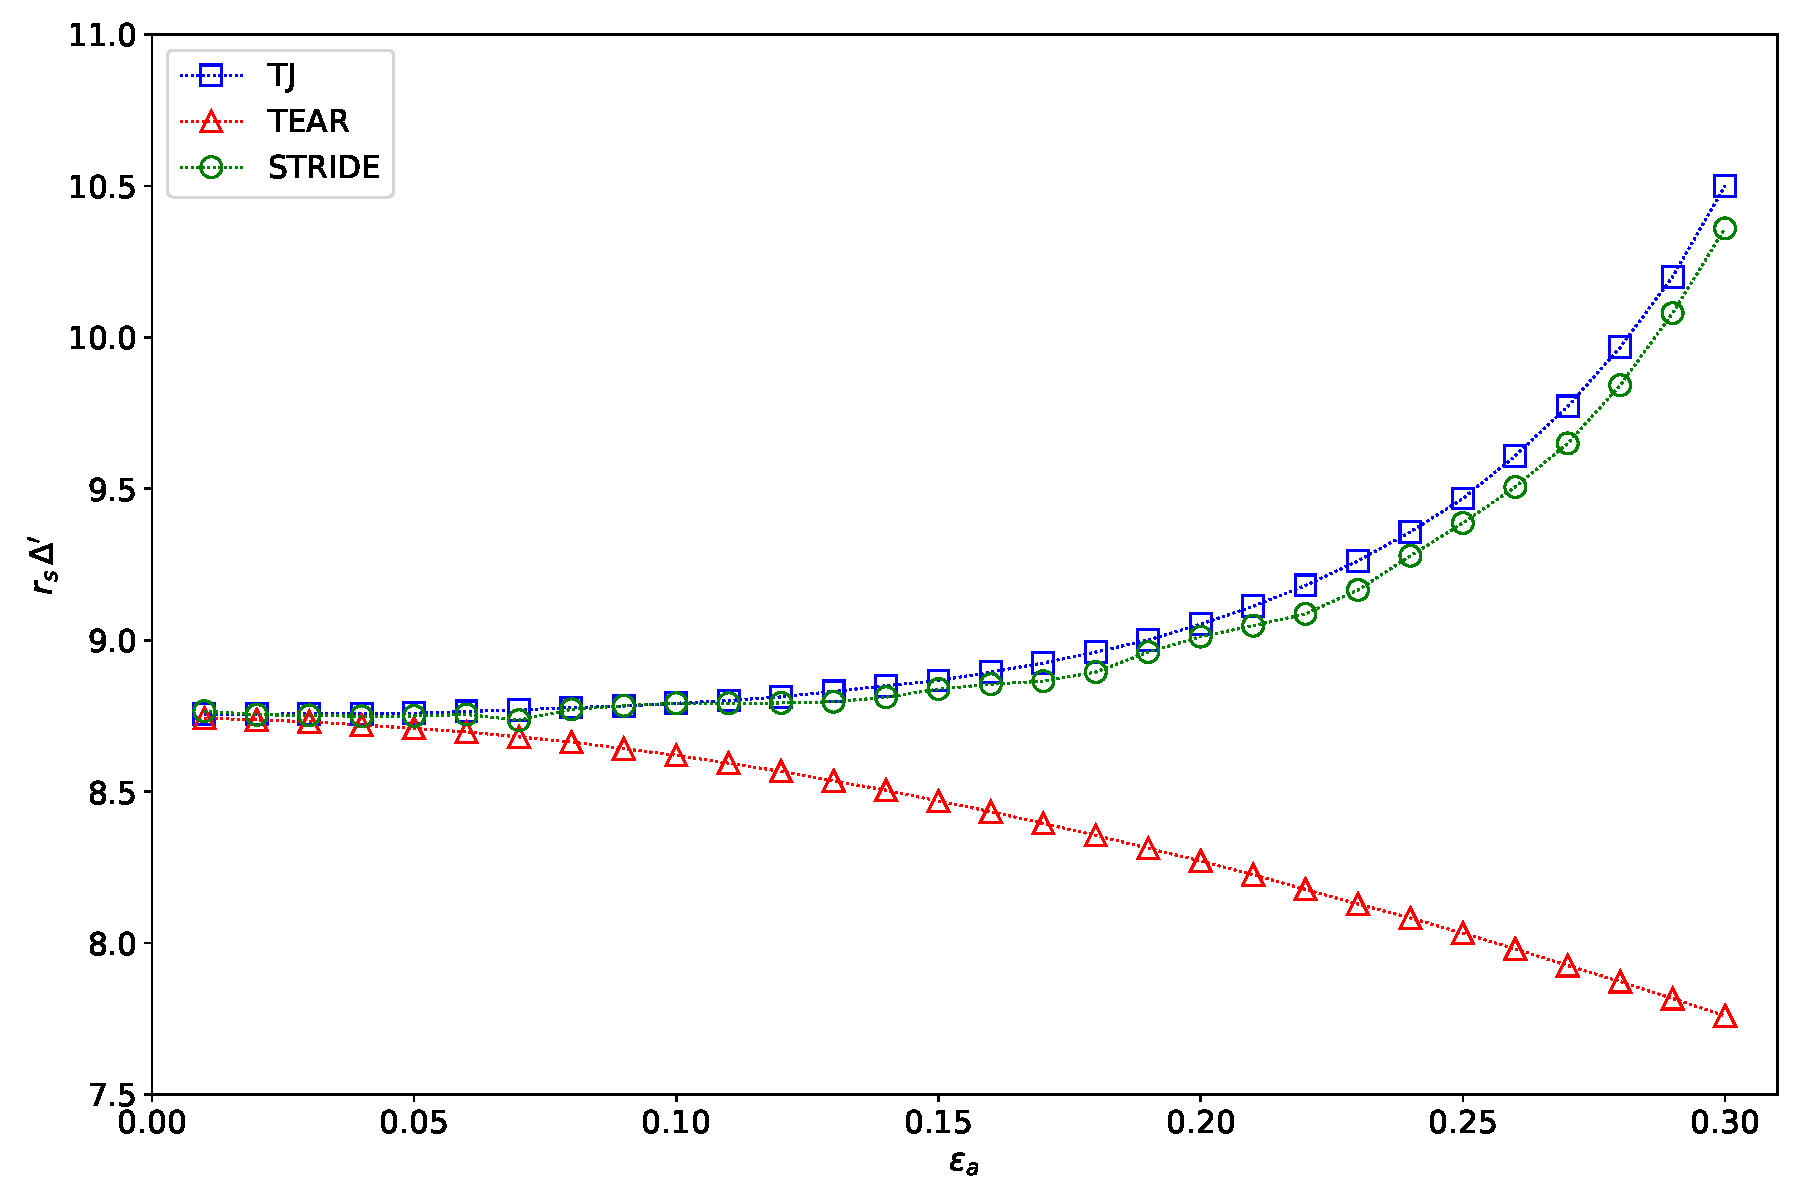
\includegraphics[width=\textwidth]{Test1.pdf}}
\caption{Test 1: $q_0=1.1$, $q_a=2.6$. Variation of 2/1 tearing stability index with inverse-aspect ratio.}
\end{figure}

\begin{figure}
\centerline{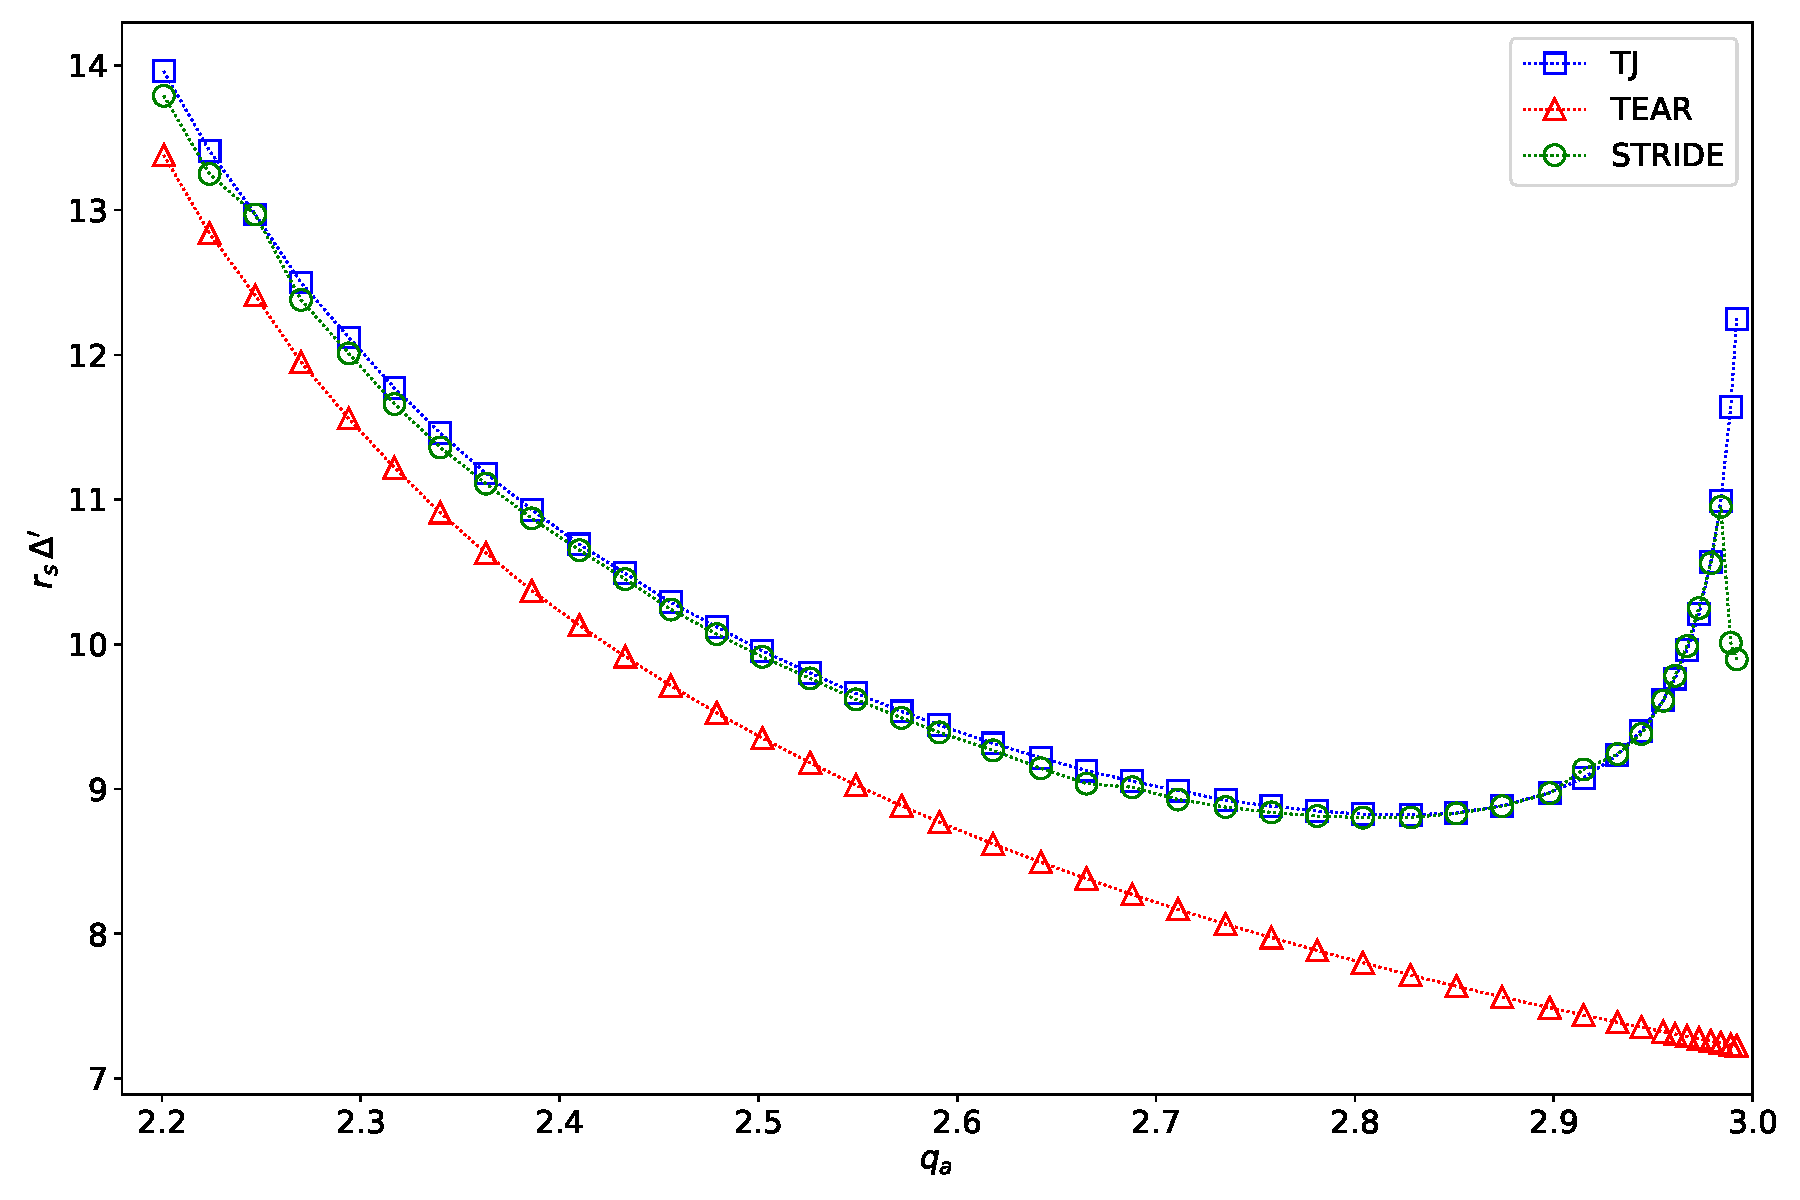
\includegraphics[width=\textwidth]{Test2.pdf}}
\caption{Test 2: $q_0=1.1$, $\epsilon_a=0.05$. Variation of 2/1 tearing stability index with edge safety-factor.}
\end{figure}

\begin{figure}
\centerline{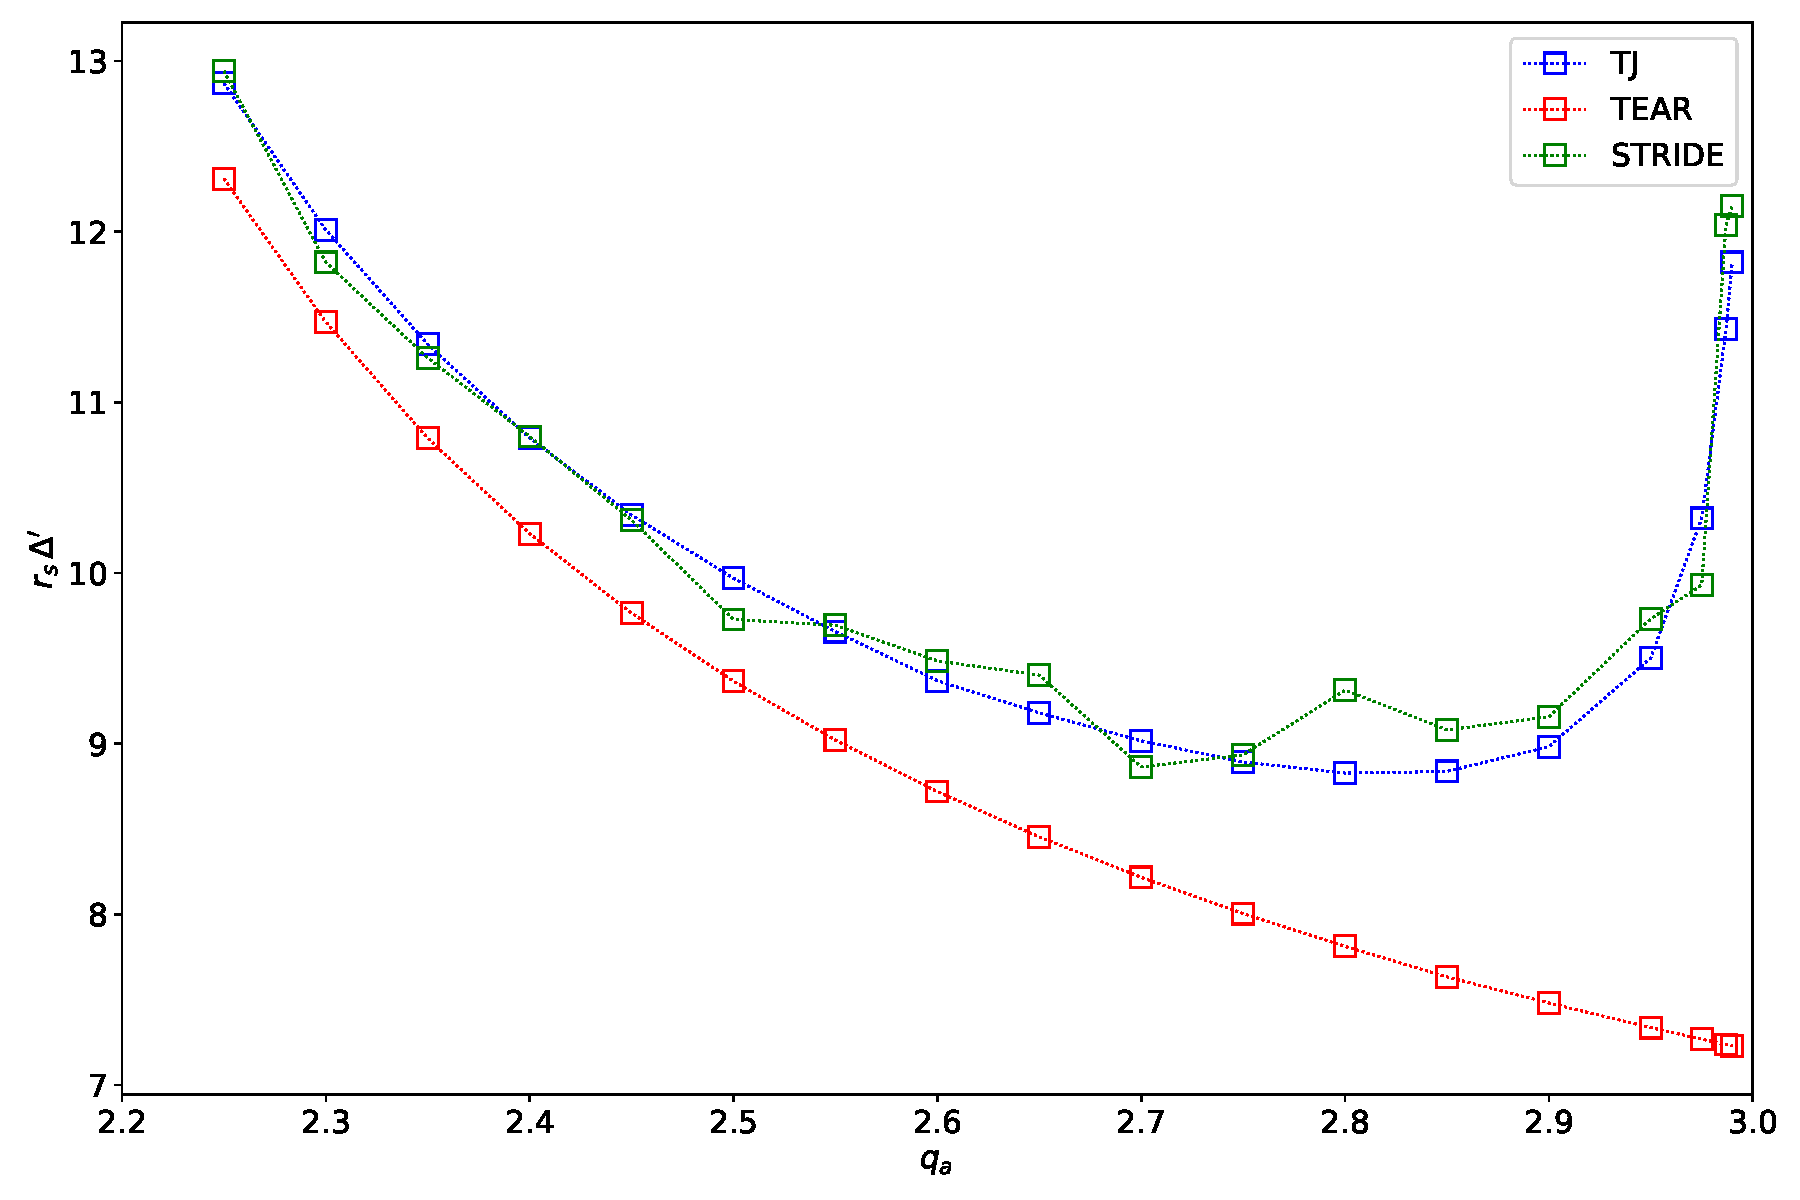
\includegraphics[width=\textwidth]{Test3.pdf}}
\caption{Test 3:  $q_0=1.1$, $\epsilon_a=0.2$. Variation of 2/1 tearing stability index with edge safety-factor.}
\end{figure}

\begin{figure}
\centerline{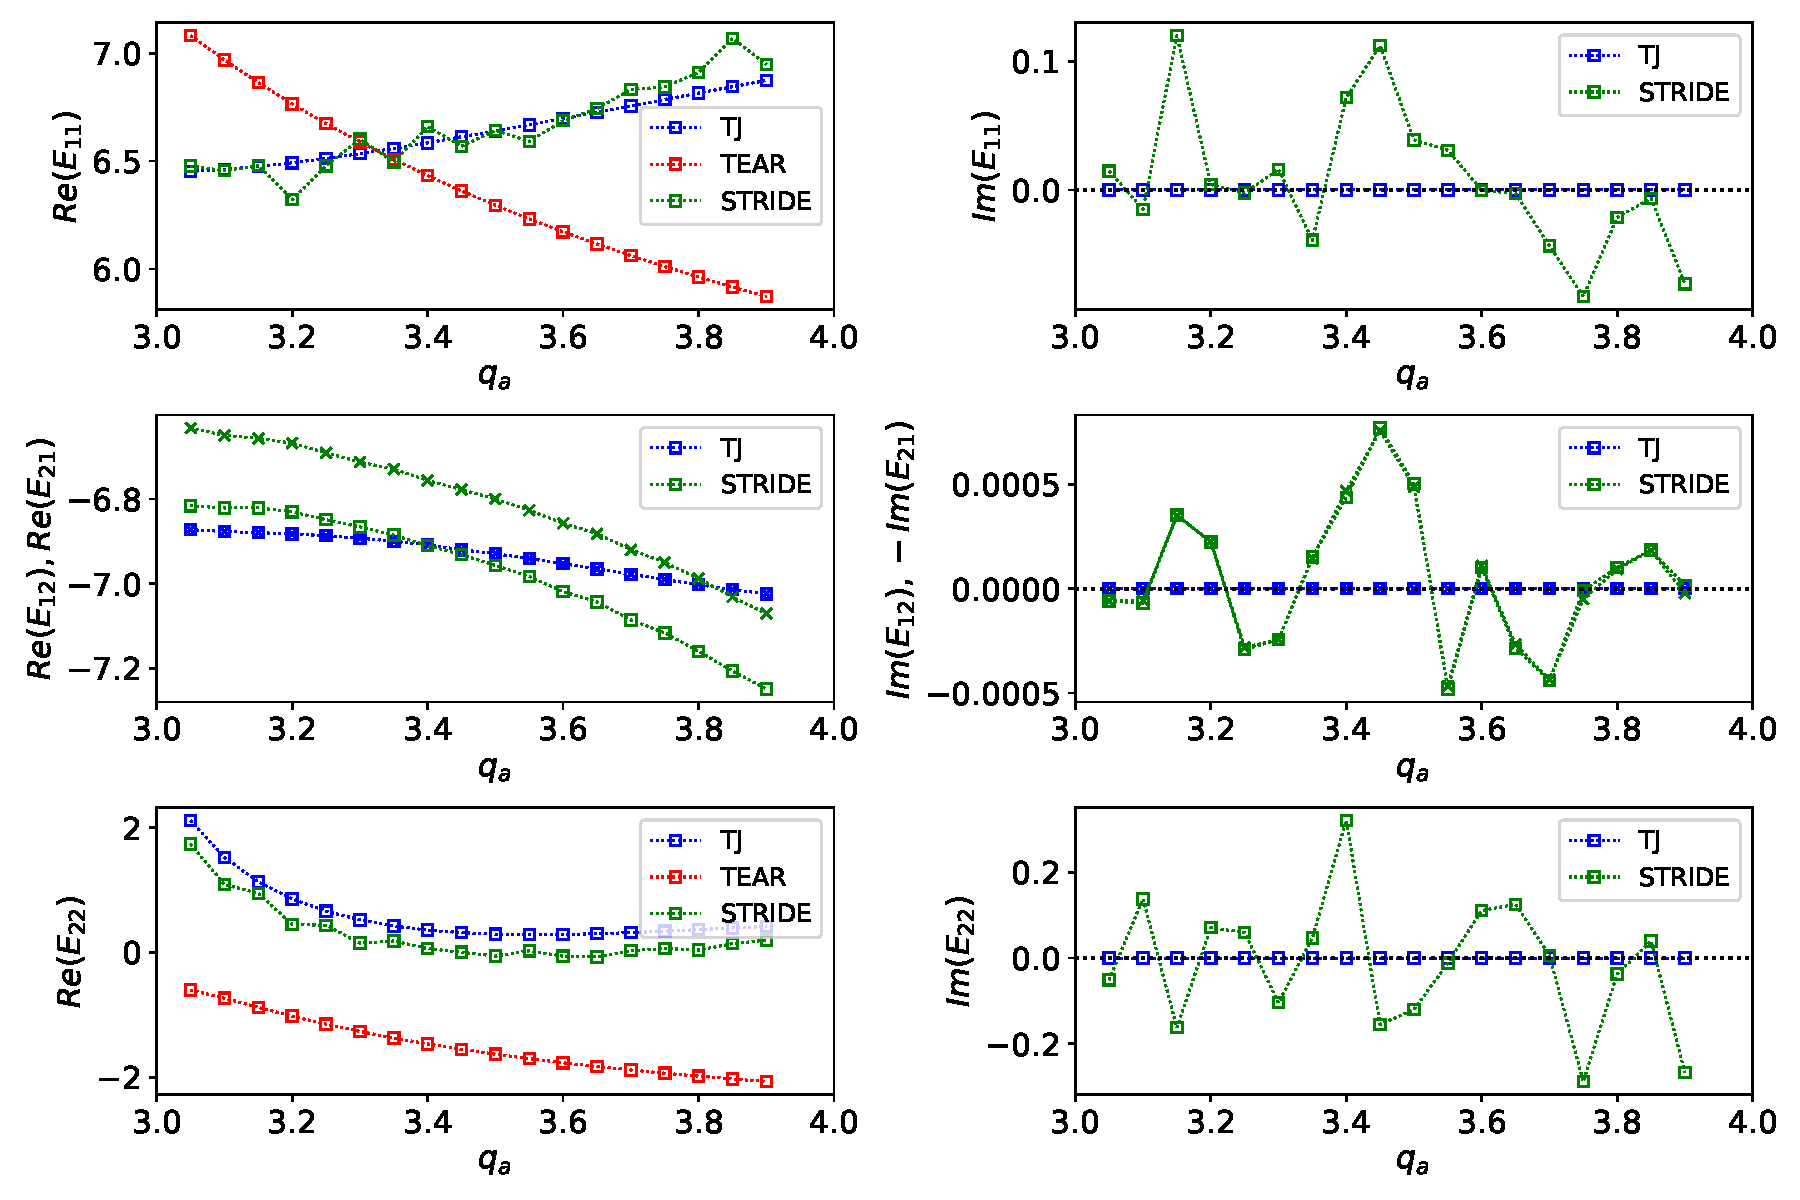
\includegraphics[width=\textwidth]{Test4.pdf}}
\caption{Test 4:  $q_0=1.1$, $\epsilon_a=0.3$. Variation of elements of tearing stability matrix with edge safety-factor.}
\end{figure}




\end{document}

